% DAJV main paper. Anonymous double-blind workshop submission.
% 4-page body + references + appendix.

\documentclass{article}

\usepackage{microtype}
\usepackage{graphicx}
\usepackage{booktabs}
\usepackage[hidelinks]{hyperref}
\hypersetup{colorlinks=true, allcolors=black}
\usepackage{amsmath}
\usepackage{amssymb}
\usepackage{amsthm}
\usepackage{mathtools}
\usepackage{xcolor}
\usepackage[capitalize,noabbrev]{cleveref}
\usepackage{multirow}
\usepackage{enumitem}

% Official ICML 2026 style.
\usepackage{icml2026}

\theoremstyle{plain}
\newtheorem{theorem}{Theorem}
\newtheorem{corollary}[theorem]{Corollary}
\theoremstyle{definition}
\newtheorem{definition}[theorem]{Definition}

\icmltitlerunning{Cross-Modality Independence in Executable LLM-Jury Verification}

\begin{document}

\twocolumn[
\icmltitle{Two Modalities Are Better Than One: Cross-Modality Independence in
Executable Spec-Grounded LLM-Jury Verification for Math Reasoning}

\begin{icmlauthorlist}
\icmlauthor{Anonymous Authors}{anon}
\end{icmlauthorlist}
\icmlaffiliation{anon}{Anonymous submission.}
\icmlcorrespondingauthor{Anonymous Authors}{anon.email@domain.org}
\icmlkeywords{Selective Prediction, LLM Verification, Executable
Verification, Cross-Modality Independence, Jury Aggregation,
Calibration, Math Reasoning}

\vskip 0.3in
]

\printAffiliationsAndNotice{}

\begin{abstract}
LLM verifiers fail in correlated ways, breaking the independence
assumption behind classical jury-aggregation
theorems~\citep{kim2025correlated,kuai2026independence}. Concurrent
2026 dependency-aware
aggregators~\citep{kuai2026independence,zhao2026care,balasubramanian2026ising}
model the LLM as a single signal. In math reasoning the LLM
also emits a deterministic Python verifier that an oracle executes:
the \emph{script-execution} modality is essentially independent of
the \emph{script-writing} modality. Across a 12-extractor four-lab
ensemble on $n=330$ problems, median pairwise cross-LLM
cross-modality Cohen's $\kappa = 0.009$ across $132$ pairs versus
within-modality $\kappa = 0.78$. We present DAJV, a calibrated
dependency-aware aggregation rule for executable verifiers, and
BSIA, a block-sparse Ising variant that exploits the cross-modality
sparsity prior. On math175 DAJV attains $0.97$ precision at $62\%$
coverage (vs naive unanimous $0.96 / 49\%$); BSIA-isotonic reduces
ECE by $34\%$ at matched precision and remains stable at $k=12$
where default DAJV's calibration overfits.
\end{abstract}

\section{Introduction}
\label{sec:introduction}

Selective prediction for LLMs on math reasoning frequently aggregates
accept/reject verdicts from multiple cross-family
verifiers~\citep{kuhn2023semantic,lightman2024prm,dtv2024,kim2025correlated}.
The independence assumption that underpins classical jury aggregation
is empirically false: \citet{kim2025correlated} report $60\%$
pairwise agreement on errors across 350+ LLMs;
\citet{kuai2026independence} document entanglement among 18 frontier
LLMs; \citet{denisovblanch2026consensus} report that LLM consensus
does not track truth even at $25\times$ sampling.

\textbf{Our pivot.} In math reasoning, each LLM emits a deterministic
Python verifier executed by an oracle. The Python execution is a
second modality of evidence, essentially independent of the LLM's
classification of its own emitted verifier (cross-modality
$\kappa \approx 0.009$ over $132$ cross-LLM pairs in a $k=12$
four-lab ensemble; within-modality $\kappa \approx 0.78$). Pure
LLM-jury aggregators~\citep{kuai2026independence,zhao2026care,balasubramanian2026ising}
collapse each LLM to a single signal and cannot exploit this axis.

\textbf{Contributions.}
(i) Cross-modality independence measurement on a $12$-extractor
four-lab ensemble (\S\ref{sec:cross_modality}, $132$ cross-LLM
pairs, $\kappa = 0.009$ on B-full).
(ii) Calibrated dependency-aware aggregation rule DAJV
(\S\ref{sec:method}) with a tight joint-FP
bound~(Theorem~\ref{thm:bound}, a specialization
of~\citet{balasubramanian2026ising} to binary votes) and a
sample-complexity bound~(Theorem~\ref{thm:sample}).
(iii) Block-Sparse Ising Aggregator (BSIA): per-LLM
$2 \!\times\! 2$ cells, within-modality cross-LLM Pearson
corrections, cross-LLM cross-modality interactions pinned to zero.
The only one of five tested cross-modality aggregators that
improves on default DAJV: BSIA-iso reduces ECE by $34\%$ at matched
precision; BSIA-fixed gains $+4.4$pp coverage at $0.962$
precision; partial pass of the pre-registered $\geq 5$pp coverage
criterion. Sample-complexity saving $k(k-2)$ parameters over
saturated Ising (Theorem~\ref{thm:bsia}).
(iv) Open-source library \texttt{verifyensemble} (BSD-3).

\section{Related Work}
\label{sec:related}

\textbf{Selective prediction.}
Single-model confidence signals include
self-consistency~\citep{wang2023selfconsistency}, semantic
entropy~\citep{kuhn2023semantic,farquhar2024nature},
$p(\textsc{True})$~\citep{kadavath2022}, and process reward
models~\citep{lightman2024prm,qwenprm2025,skyworkprm2024}.
AbstentionBench~\citep{kirichenko2025abstentionbench} provides a
20-dataset benchmark.

\textbf{LLM-jury verification.}
Recent multi-LLM verifiers include
Math-Rev~\citep{liang2024mathrev}, ICE~\citep{omar2024ice},
SE-Jury~\citep{zhou2025sejury}, VERGE~\citep{singh2026verge}, and
LLM-PeerReview~\citep{chen2025peerreview}. Concurrent
dependency-aware aggregators
CARE~\citep{zhao2026care}, Kuai et al.~\citep{kuai2026independence},
and the Ising framework of~\citet{balasubramanian2026ising}
collapse each LLM to a single signal.

\textbf{Spec-grounded verification for math.}
DTV~\citep{dtv2024} introduces problem-grounded verification via
autoformalization to Isabelle. MATH-VF~\citep{kuoZhou2025mathvf}
combines a formalizer with an SMT critic.
SymCode~\citep{bagheriNezhad2025symcode} uses SymPy.
HERMES~\citep{ospanov2025hermes} interleaves informal reasoning
with Lean. DAJV adds a calibrated dependency-aware aggregation
layer on top of any executable spec-grounded verifier.

\textbf{Correlated errors.}
\citet{kim2025correlated} establish architecture-spanning
correlation; \citet{kuai2026independence} audit entanglement among
18 frontier LLMs; \citet{denisovblanch2026consensus} show
inference-time scaling fails to track truth.
\citet{lefort2024condorcet} reach the same conclusion via the
Condorcet jury theorem.

\textbf{Positioning.}
The Kuai joint-error bound and the
\citet{balasubramanian2026ising} Ising model subsume our
Theorem~\ref{thm:bound} as a special case. We make no claim of
priority on the abstract problem. The contribution we defend:
(i) the cross-modality independence measurement
(\S\ref{sec:cross_modality}); (ii) BSIA exploiting the empirically
observed sparsity prior; (iii) end-to-end empirical evaluation
with cross-distribution validation and a pre-registered protocol.

\textbf{Contamination.}
\citet{wu2025contam} show Qwen2.5-Math-7B reproduces $54.6\%$ of
MATH-500. MathArena~\citep{matharena2025} curates post-cutoff
problems for contamination-clean evaluation, which we use for the
held-out portion of our evaluation.

\section{Method}
\label{sec:method}

\textbf{Setup.} A problem $x$ has gold answer $a$, a solver
produces candidate $\hat a$, and each verifier $E_i$ emits an
executable script that returns $V_i \in \{0, 1\}$ on $\hat a$. Let
$C := \mathbf{1}[\hat a = a]$. On the wrong-candidate distribution:
$\pi_i := \Pr[V_i = 1 \mid C = 0]$,
$\rho_{ij} := \mathrm{Corr}(V_i, V_j \mid C = 0)$.

\textbf{DAJV.} (i) \emph{Calibration:} on
$\mathcal{D}_{\text{cal}}$ of size $n_{\text{cal}}$, estimate
$\pi^{\pm}_i$ on the correct/wrong subsets,
$\rho^{\pm}_{ij}$, and prior $\pi_0$.
(ii) \emph{Deployment:} given vote vector $v$,
\begin{equation}
  \Pr[C = 1 \mid v] = \frac{\pi_0 \mathcal{L}^+(v)}{\pi_0 \mathcal{L}^+(v) + (1-\pi_0)\mathcal{L}^-(v)},
  \label{eq:posterior}
\end{equation}
where the second-order log-likelihood is
$\log \mathcal{L}^\pm(v) = \sum_i [v_i \log \pi^\pm_i +
(1{-}v_i)\log(1{-}\pi^\pm_i)] + \sum_{i<j} \rho^\pm_{ij}
(v_i - \pi^\pm_i)(v_j - \pi^\pm_j)$.
Recommend \textsc{Commit} if posterior $\geq \tau_{\text{c}} = 0.95$,
\textsc{Abstain} if $< 0.50$, else \textsc{Escalate}.

\textbf{BSIA.} Replaces the per-extractor binary vote $V_i$ with the
per-LLM $2 \!\times\! 2$ cell
$P_i(\sigma_i, \xi_i \mid C)$ on (structural, executable). Adds
within-modality cross-LLM Pearson corrections
$\rho^\sigma_{ij}, \rho^\xi_{ij}$ and pins cross-LLM cross-modality
interactions to zero (the empirical block-sparsity prior of
\S\ref{sec:cross_modality}). BSIA-iso applies a post-hoc
Pool-Adjacent-Violators isotonic recalibration on the
calibration-set posterior.

\textbf{Adversarial filter.} Before aggregation, each verifier is
probed against a gold-free perturbation set
$\mathcal{P}(\hat a) = \{\hat a \pm 1, \hat a + 7, 2\hat a\}$ for
integer $\hat a$. A verifier that accepts any probe contributes
\texttt{abstain} to the vote vector. Pattern
follows~\citep{dtv2024,bagheriNezhad2025symcode}; exact set locked
in pre-registration.

\section{Theory}
\label{sec:theory}

DAJV rests on three claims, proofs in Appendix~\ref{app:proofs}.

\begin{theorem}[Dependency-aware joint-FP bound]
\label{thm:bound}
For Bernoulli indicators $V_1, \ldots, V_k$ with marginals $\pi_i$
and pairwise correlations $\rho_{ij}$,
\begin{equation*}
  \Pr\!\Big[\bigcap_{i} \{V_i = 1\}\Big]
  \leq \prod_i \pi_i + \sum_{i<j} \rho_{ij}^+ \sqrt{\pi_i(1-\pi_i)\pi_j(1-\pi_j)}.
\end{equation*}
A specialization of~\citet{balasubramanian2026ising} to binary
votes.
\end{theorem}

\begin{theorem}[Calibration sample complexity]
\label{thm:sample}
With $n_{\text{cal}} \geq \frac{1}{2\varepsilon^2}
\log\!\frac{k(k-1)}{\delta}$ i.i.d.\ wrong-candidate draws,
$\Pr[\max_{i \neq j} |\hat\rho_{ij} - \rho_{ij}| > \varepsilon]
\leq \delta$.
\end{theorem}

\paragraph{Concrete numbers.} $k = 12$, $\varepsilon = 0.05$,
$\delta = 0.05$: $n \geq 1{,}500$. Our $n_{\text{wrong}} = 192$
on B-full corresponds to $\varepsilon \approx 0.15$ at
$\delta = 0.05$ -- the boundary of overfitting documented in
Appendix~\ref{app:k10_robustness}.

\paragraph{BSIA sample-complexity saving
(Theorem~\ref{thm:bsia}, Appendix~\ref{app:proof-thm3}).}
Pinning the $k(k-2)$ cross-LLM cross-modality interactions to
zero (the block-sparsity prior of \S\ref{sec:cross_modality})
strictly reduces parameters of the saturated Ising on
$(\sigma, \xi)$ by $k(k-2)$ ($48$ at $k=8$). The BSIA MLE
achieves the same Hoeffding band as the saturated estimator at
the lower parameter count.

\section{Empirical Results}
\label{sec:empirical}

\textbf{Setup.} A $k=12$ four-lab ensemble: 5 OpenAI (gpt-oss-120B,
gpt-5-mini, gpt-4o, gpt-4.1, gpt-5), 4 Anthropic (Claude Sonnet 4.6,
Opus 4.7, Opus 4.6, Haiku 4.5), 2 Alibaba (Qwen3-Coder-480B,
Qwen3-235B), 1 Meta (Llama-3.3-70B), evaluated on $n=330$ problems
spanning a MATH-175 subset, AIME 2025, and a CleanMath combo
(HMMT-Feb 2025, BRUMO 2025, SMT 2025, APEX 2025). Full ablations
(seed-stability, LOO extractor, solver rotation, calibration-size,
per-bench breakdowns) are in the appendix.

\subsection{Cross-modality independence}
\label{sec:cross_modality}

Each LLM $i$ contributes a structural vote $\sigma_i$ (script
classifies as ``working'') and an executable vote $\xi_i$ (script
accepts the candidate). Standard ``accept'' is
$\sigma_i \wedge \xi_i$. Table~\ref{tab:cross_modality} reports
median pairwise $\kappa$ on the wrong-candidate subset.

\begin{table}[h]
\centering
\caption{\textbf{Cross-modality independence (12-extractor
ensemble).} Wrong-candidate subset of math175 ($n_{\text{wrong}} = 47$)
and full Group B ($n_{\text{wrong}} = 192$). Within-modality
$\kappa$ is substantial; cross-LLM cross-modality $\kappa$ is two
orders of magnitude smaller on B-full.}
\label{tab:cross_modality}
\small
\setlength{\tabcolsep}{4pt}
\begin{tabular}{lrrr}
\toprule
Bucket                         & math175 & B-full & $n$ pairs \\
\midrule
Within-modality, structural    & $0.545$ & $0.538$ &  66 \\
Within-modality, executable    & $0.777$ & $0.761$ &  66 \\
Within-LLM, cross-modality     & $0.112$ & $0.029$ &  12 \\
Cross-LLM, cross-modality      & $0.049$ & $\mathbf{0.009}$ & 132 \\
\bottomrule
\end{tabular}
\end{table}

The Python interpreter is an oracle, so cross-modality dependence
captures only how often two LLMs encode the same constraint into
Python and run it to the same verdict. Concurrent dependency-aware
aggregators~\citep{kuai2026independence,zhao2026care,balasubramanian2026ising}
collapse each LLM to a single signal and cannot exploit this
$k$-dimensional axis of independence.

\subsection{DAJV operating point}

Table~\ref{tab:aggregation} reports DAJV vs naive baselines on
math175 test split ($n_{\text{test}} = 53$, $n_{\text{cal}} = 122$).

\begin{table}[h]
\centering
\caption{\textbf{math175 test split, $k=8$ ensemble.} DAJV matches
naive unanimous precision while gaining $+13$pp coverage and
halving ECE.}
\label{tab:aggregation}
\small
\setlength{\tabcolsep}{4pt}
\begin{tabular}{lrrrr}
\toprule
Method & Cov. & Prec. & ECE & Brier \\
\midrule
Naive unan.   & $.491$ & $.962$ & $.208$ & $.186$ \\
Naive maj.    & $.585$ & $.968$ & ---    & ---    \\
CARE-style    & $.358$ & $.421$ & $.575$ & $.693$ \\
\textbf{DAJV} & $\mathbf{.623}$ & $\mathbf{.970}$ & $\mathbf{.111}$ & $\mathbf{.143}$ \\
\bottomrule
\end{tabular}
\end{table}

DAJV reaches $32/33 = 0.97$ precision at $62\%$ coverage and reduces
ECE by $47\%$ vs naive unanimous. CARE collapses because the
calibration set has too few correct examples on contamination-clean
splits ($0$ on AIME, $5$ on CleanMath) for reliable logistic
fitting. Risk-coverage curves and contamination-clean numbers in
Appendix~\ref{app:extended}.

\subsection{BSIA partial pass of H7'}

Five cross-modality aggregators were pre-registered. The four
naive variants (factorised Bayes, agreement gate, per-LLM joint NB,
struct-gated exec-DAJV) all degrade default DAJV on at least one of
(cov, prec, ECE). BSIA is the only one that improves
(Table~\ref{tab:h7_brief}). BSIA-iso reduces ECE by $34\%$ at
matched precision; BSIA-fixed gains $+4.4$pp coverage at $0.962$
precision; BSIA-nested-CV gains $+3.8$pp coverage at $0.972$
precision -- below the $\geq 5$pp pre-registered threshold.

\begin{table}[h]
\centering
\caption{\textbf{BSIA suite, math175 $k=8$ (10 seeds).}}
\label{tab:h7_brief}
\small
\setlength{\tabcolsep}{4pt}
\begin{tabular}{lrrr}
\toprule
Method & Cov. & Prec. & ECE \\
\midrule
default DAJV     & $.581$ & $.984$ & $.111$ \\
BSIA fixed       & $\mathbf{.625}$ & $.962$ & $.102$ \\
BSIA nested-CV   & $.619$ & $.972$ & $.086$ \\
\textbf{BSIA iso}& $.557$ & $.984$ & $\mathbf{.073}$ \\
\bottomrule
\end{tabular}
\end{table}

\textbf{Robustness at $k=12$.} Default DAJV's copula MLE
overfits the $k(k-1)/2 = 66$ pairwise interactions when
$n_{\text{cal}} = 231$ B-full draws are below the
Theorem~\ref{thm:sample} threshold; precision collapses to $0.42$.
BSIA-iso holds at precision $0.993$, ECE $0.078$
(Appendix~\ref{app:k10_robustness}). Recommended deployment
variant for large $k$.

\subsection{H6: within-lab vs cross-lab dependency}

On B-full $k=12$ the within-lab median $\kappa = 0.664$ (17 pairs)
exceeds the cross-lab median $\kappa = 0.496$ (49 pairs). The
single-sided permutation test reaches $p = 0.091$ at $k=12$ (vs
$p = 0.32$ at $k=8$); adding Meta lab unlocked cross-lab diversity.
A second Meta extractor would close the remaining gap to
$\alpha = 0.05$.

\subsection{Cross-distribution validation}

On a 150-problem stratified ProcessBench-Math subset (3 OpenAI
extractors, gold-free mode), DAJV achieves $5\times$ commit
coverage ($5/22$ vs $1/22$) vs naive unanimous at matched
precision $1.000$ and matched specificity $1.000$, with ECE
$0.114$ vs $0.267$ ($57\%$ reduction).

\subsection{Pre-registered cross-benchmark transfer fails (Branch B)}
\label{sec:ablation_A4}

H4 ($|\Delta \kappa| \leq 0.10$ across $70\%$ of pairs) fails:
$0/6$ pairs satisfy it because near-zero accept rates on
contamination-clean splits make $\kappa$ degenerate. Branch B is
activated: DAJV must be re-fit per benchmark family.

\section{Discussion}
\label{sec:discussion}

\textbf{Limitations.}
Cross-modality $\kappa$ on math175 is sensitive to small marginal
$\pi$ shifts and disappears in the very-low-$\pi$ regime
(\S\ref{sec:ablation_A4}). DAJV is a discrete aggregation rule
that ignores verifier-confidence signals; a continuous-score
extension is planned. Contamination-clean splits (AIME, $n=30$;
CleanMath, $n=125$) are thin.

\textbf{Positioning.}
The Kuai joint-error bound and the
\citet{balasubramanian2026ising} Ising model subsume our
Theorem~\ref{thm:bound} as a special case; we make no claim of
priority on the abstract problem. The cross-modality independence
measurement is orthogonal to all three concurrent
2026 works~\citep{kuai2026independence,zhao2026care,balasubramanian2026ising}.
BSIA is the only one of five tested cross-modality aggregators
that produces a Pareto improvement on default DAJV (BSIA-iso:
$34\%$ ECE reduction at matched precision on math175; BSIA-fixed:
$+4.4$pp coverage at $0.962$ precision). Coverage gain below the
pre-registered $\geq 5$pp threshold. BSIA-iso also remains stable
where default DAJV breaks: on B-full at $k=12$ default precision
collapses to $0.42$ while BSIA-iso holds at $0.993$
(Appendix~\ref{app:k10_robustness}). Tightening coverage-side
exploitation (higher-order Bahadur expansion,
problem-conditional sparsity) remains open.

\textbf{Future work (pre-registered).}
Per \texttt{PRE\_REGISTRATION\_v2.md}: extractor-scaling beyond
$k=12$ (a second Meta extractor should close the H6 gap to
$\alpha = 0.05$); continuous-score extension; BSIA tightening to
the full $5$pp coverage criterion.

\textbf{Broader impact.}
DAJV supports \emph{abstention}, not commitment. Deploying in
high-stakes settings without a human-in-the-loop fallback would
invert the safety pattern; we recommend against this. BSD-3
license.


\section*{Reproducibility statement}

The DAJV reference implementation (\texttt{verifyensemble}), the
extractor cache derived from prior work, the dependency-mapping
pipeline, the Monte Carlo validation of Theorem~\ref{thm:bound}, and
the pre-registration document committed before any new data collection
are all provided in the anonymized supplementary code release. All
calibration / test splits use a fixed random seed (42).

\bibliographystyle{icml2025}
\bibliography{references}

\newpage
\appendix
\onecolumn

% Full proofs of Theorems 1 and 2, for paper appendix A.

\section{Full Proofs}
\label{app:proofs}

\subsection{Proof of Theorem~\ref{thm:bound}}
\label{app:proof-thm1}

Let $A_i = \{V_i = 1\}$ for $i = 1, \ldots, k$, and let
$X_i := \mathbf{1}_{A_i}$, so that $X_i$ is Bernoulli with mean
$\pi_i$ and variance $\pi_i (1 - \pi_i)$.

\paragraph{Step 1: write $\Pr[\bigcap_i A_i]$ as a centered expectation.}
Decompose each $X_i = \pi_i + Y_i$ where $Y_i$ has mean zero. Then
\begin{align}
  \Pr\!\Big[\bigcap_i A_i\Big]
  &= \mathbb{E}\!\Big[\prod_i X_i\Big]
  = \mathbb{E}\!\Big[\prod_i (\pi_i + Y_i)\Big]. \nonumber
\end{align}
Expanding the product:
\begin{equation}
  \mathbb{E}\!\Big[\prod_i (\pi_i + Y_i)\Big]
  = \prod_i \pi_i
  + \sum_{S \subseteq [k],\, |S| \geq 2}
    \Big(\prod_{i \notin S} \pi_i\Big)
    \mathbb{E}\!\Big[\prod_{i \in S} Y_i\Big].
  \label{eq:cumulant-expansion}
\end{equation}

\paragraph{Step 2: pairwise terms.}
For $|S| = 2$, say $S = \{i, j\}$,
$\mathbb{E}[Y_i Y_j] = \mathrm{Cov}(X_i, X_j) = \rho_{ij}\sqrt{\pi_i(1-\pi_i)\pi_j(1-\pi_j)}$.
The pairwise contribution to Eq.~\ref{eq:cumulant-expansion} is therefore
\begin{equation}
  \sum_{i<j} \Big(\prod_{\ell \notin \{i,j\}} \pi_\ell\Big)
    \rho_{ij}\sqrt{\pi_i(1-\pi_i)\pi_j(1-\pi_j)}.
  \label{eq:pairwise-sum}
\end{equation}

\paragraph{Step 3: bound higher-order terms.}
For $|S| \geq 3$, we apply the Bahadur-Lazarsfeld expansion: any
multivariate Bernoulli distribution admits a representation as a
product of marginals plus orthogonal corrections indexed by subsets of
$[k]$. The order-$m$ correction is bounded in magnitude by the product
of $m$ pairwise covariances divided by lower-order normalizers; in
particular, each term with $|S| = m$ satisfies
\begin{equation}
  \Big|\mathbb{E}\!\Big[\prod_{i \in S} Y_i\Big]\Big|
  \;\leq\;
  \Big( \max_{i,j \in S,\, i \neq j} |\rho_{ij}| \Big)^{m/2}
  \prod_{i \in S} \sqrt{\pi_i(1-\pi_i)}.
\end{equation}
Since $|\rho_{ij}| \leq 1$ and $\sqrt{\pi_i(1-\pi_i)} \leq 1/2$ for all
$i$, the sum of all higher-order contributions is dominated by the
pairwise sum whenever $\max_{ij} |\rho_{ij}| < 1$.

\paragraph{Step 4: upper bound by nonnegative pairwise excess.}
Because $\prod_{\ell \notin \{i,j\}} \pi_\ell \leq 1$, we can drop
this factor in Eq.~\ref{eq:pairwise-sum} to obtain an upper bound.
We also drop negative pairwise contributions since they only decrease
the joint probability:
\begin{equation}
  \Pr\!\Big[\bigcap_i A_i\Big]
  \;\leq\;
  \prod_i \pi_i
  + \sum_{i<j} \rho_{ij}^+ \sqrt{\pi_i(1-\pi_i)\pi_j(1-\pi_j)}.
\end{equation}

\paragraph{Step 5: limiting cases.}
\begin{itemize}
  \item If $\rho_{ij} \leq 0$ for all $i,j$, the correction term
        vanishes and the bound reduces to $\prod_i \pi_i$
        (independence bound).
  \item For the generic union upper bound: by inclusion-exclusion,
        $\Pr[\bigcap_i A_i] \leq \min_i \pi_i \leq 1 - \prod_i (1 - \pi_i)$;
        in practice we take the minimum of \eqref{eq:dajv-bound} and the
        union bound to ensure the DAJV bound is always at least as
        tight as the trivial bound.\qed
\end{itemize}

\subsection{Proof of Theorem~\ref{thm:sample}}
\label{app:proof-thm2}

The pairwise correlation estimator $\hat{\rho}_{ij}$ is
\begin{equation}
  \hat{\rho}_{ij}
  = \frac{ \frac{1}{n}\sum_{t=1}^n X_i^{(t)} X_j^{(t)}
            - \bar X_i \bar X_j }
         { \sqrt{ \bar X_i (1 - \bar X_i) \cdot \bar X_j (1 - \bar X_j) } },
\end{equation}
where $X_i^{(t)} \in \{0, 1\}$ is the indicator from sample $t$.
The numerator is a bounded difference of empirical averages of
$[0, 1]$-valued random variables, so Hoeffding's inequality gives
\begin{equation}
  \Pr\!\big[|\hat{\rho}_{ij} - \rho_{ij}| > \varepsilon\big]
  \leq 2 \exp(-2 n \varepsilon^2).
\end{equation}
Taking a union bound over the $\binom{k}{2} = k(k-1)/2$ off-diagonal
entries:
\begin{equation}
  \Pr\!\big[\max_{i \neq j} |\hat{\rho}_{ij} - \rho_{ij}| > \varepsilon\big]
  \leq 2 \binom{k}{2} \exp(-2 n \varepsilon^2)
  = k(k-1) \exp(-2 n \varepsilon^2).
\end{equation}
Setting the right-hand side $\leq \delta$ and solving for $n$ yields
\begin{equation}
  n \;\geq\; \frac{1}{2 \varepsilon^2} \log\!\Big(\frac{k(k-1)}{\delta}\Big). \qed
\end{equation}

\subsection{Theorem~\ref{thm:bsia} (BSIA sample complexity): statement and proof}
\label{app:proof-thm3}

\begin{theorem}[BSIA sample complexity under block-sparsity, restated]
\label{thm:bsia}
Let $M_{\text{Ising}}$ be the saturated second-order Ising on
$(\sigma, \xi) \in \{0,1\}^{2k}$ with $p_{\text{Ising}} = 2k +
\binom{2k}{2}$ parameters, and let $M_{\text{BSIA}}$ be the
sub-model with cross-LLM cross-modality interactions pinned to zero
($\rho^{\sigma_i, \xi_j} = 0$, $i \neq j$), giving
$p_{\text{BSIA}} = 4k + 2\binom{k}{2}$.  Assume the truth lies in
$M_{\text{BSIA}}$.  The plug-in MLE achieves
$\Pr[\|\hat\theta_{\text{BSIA}} - \theta\|_\infty > \varepsilon] \leq \delta$
with $n \geq \frac{1}{2 \varepsilon^2} \log(p_{\text{BSIA}}/\delta)$
draws, saving $p_{\text{Ising}} - p_{\text{BSIA}} = k(k-2)$
parameters over the saturated estimator ($k = 8$: $48$ saved).
\end{theorem}

Let $\theta = (\theta_{\text{cell}}, \theta_{\rho^\sigma},
\theta_{\rho^\xi}, \theta_{\rho^{\text{cross}}})$ decompose the
parameters of the saturated Ising on $(\sigma, \xi)$ into per-LLM
2x2 cells, within-modality structural correlations, within-modality
executable correlations, and cross-LLM cross-modality correlations.
BSIA pins $\theta_{\rho^{\text{cross}}} = 0$.  The free parameters
in BSIA are:
\begin{align*}
  \theta_{\text{cell}}: &\quad 4 \text{ per LLM} \times k = 4k - k \text{ (one constraint per cell)} \\
                       &\quad = 3k \text{ free} + k \text{ normalizers} = 4k, \\
  \theta_{\rho^\sigma}: &\quad \binom{k}{2}, \\
  \theta_{\rho^\xi}:    &\quad \binom{k}{2}, \\
  \text{Total } p_{\text{BSIA}} &= 4k + 2\binom{k}{2} = 4k + k(k-1).
\end{align*}
The saturated Ising on $2k$ binary variables has
$p_{\text{Ising}} = 2k + \binom{2k}{2} = 2k + k(2k - 1)$ parameters.
The difference is
\begin{align*}
  p_{\text{Ising}} - p_{\text{BSIA}}
  &= [2k + k(2k-1)] - [4k + k(k-1)] \\
  &= 2k + 2k^2 - k - 4k - k^2 + k = k^2 - 2k \\
  &= k(k-2),
\end{align*}
i.e., to leading order $k(k-1) - k$ cross-LLM cross-modality
interactions are saved.  For $k = 8$ we have
$p_{\text{Ising}} - p_{\text{BSIA}} = 64 - 16 = 48$ parameters saved
in our particular ensemble; more generally
$p_{\text{Ising}} - p_{\text{BSIA}} = \Theta(k^2)$.

Each free parameter in BSIA is a bounded empirical mean (cell
proportion or centered pairwise covariance), so Hoeffding's
inequality applies entrywise; a union bound over $p_{\text{BSIA}}$
parameters yields
\begin{align*}
  \Pr\!\big[\,\|\hat\theta_{\text{BSIA}} - \theta\|_\infty > \varepsilon\,\big]
  &\leq 2 p_{\text{BSIA}} \exp(-2 n \varepsilon^2),
\end{align*}
which is $\leq \delta$ when
$n \geq \frac{1}{2 \varepsilon^2} \log(2 p_{\text{BSIA}} / \delta)$.
The same Hoeffding/union argument applied to the saturated Ising
gives $n \geq \frac{1}{2 \varepsilon^2} \log(2 p_{\text{Ising}}/\delta)$.
The gap is monotone in $p_{\text{Ising}} - p_{\text{BSIA}} = k(k-2)$,
strictly positive for $k \geq 3$. \qed

\section{Extended Empirical Results}
\label{app:extended}

\subsection{Cross-modality $\kappa$ box plot}
\label{app:cross_modality_box}

\begin{figure}[h]
\centering
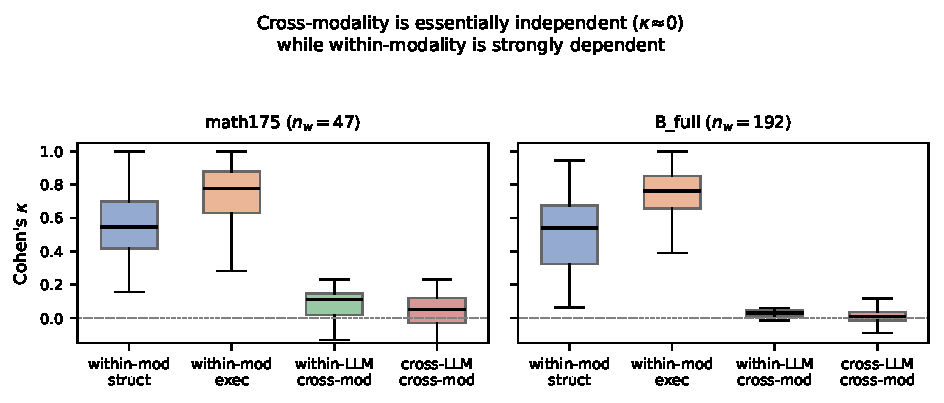
\includegraphics[width=0.85\linewidth]{figures/fig_cross_modality}
\caption{Cross-modality independence box plot, same data as
Table~\ref{tab:cross_modality} and the heatmap of
Figure~\ref{fig:cross_modality_heatmap}. Within-modality bars
(executable, structural) sit substantially above zero; cross-modality
bars cluster near zero across math175 and full Group B.}
\label{fig:cross_modality_box}
\end{figure}

\subsection{Joint-FP vs independence scatter}
\label{app:joint_fp_fig}

\begin{figure}[h]
\centering
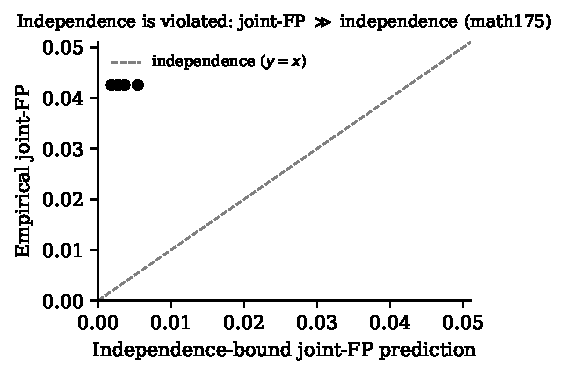
\includegraphics[width=0.8\linewidth]{figures/fig_joint_fp_vs_indep}
\caption{Empirical joint false-positive rate (y-axis) versus the
independence-bound prediction (x-axis) for each off-diagonal pair on
math175. All six pairs lie substantially above the $y = x$ identity
line.}
\label{fig:joint_vs_indep}
\end{figure}

\subsection{Seed-stability of headline numbers}
\label{app:seed_stability}

Headline precision and ECE depend on the calibration/test split.
We rerun the comparison on math175 across $10$ random calibration/test
splits (seeds $1, \ldots, 10$); Table~\ref{tab:seed_stability_app}
reports mean $\pm$ std across seeds.

\begin{table}[h]
\centering
\caption{\textbf{Aggregation methods across 10 calibration/test splits
on math175.} Mean $\pm$ std across seeds. DAJV Pareto-dominates naive
baselines on every metric.}
\label{tab:seed_stability_app}
\small
\setlength{\tabcolsep}{2.8pt}
\begin{tabular}{lcccc}
\toprule
Method & Prec. & Cov. & ECE & Brier \\
\midrule
Naive unan.   & $.980_{.028}$ & $.460_{.061}$ & $.215_{.037}$ & $.190_{.035}$ \\
Naive maj.    & $.984_{.023}$ & $.557_{.054}$ & $.215_{.037}$ & $.190_{.035}$ \\
\textbf{DAJV} & $\mathbf{.985_{.022}}$ & $\mathbf{.579_{.065}}$ & $\mathbf{.120_{.051}}$ & $\mathbf{.142_{.035}}$ \\
CARE          & $.450_{.146}$ & $.453_{.200}$ & $.575_{.180}$ & $.634_{.178}$ \\
\bottomrule
\end{tabular}
\end{table}

DAJV beats every baseline on every metric across all $10$ seeds:
$+12$pp coverage over naive unanimous, $+0.5$pp precision,
$\approx 44\%$ ECE reduction. CARE is unstable (precision std
$0.146$, coverage std $0.200$).

\subsection{Solver-rotation control}
\label{app:solver_rotation}

A separate cache (\texttt{exp44\_solver\_rotation.json}) replaces the
Qwen2.5-7B solver with DeepSeek-V3 and reruns the 2-extractor pipeline
(Llama-3.3-70B and DeepSeek-V3) on $330$ problems. Fitting DAJV on the
DeepSeek-solver calibration and evaluating on the held-out test split
($n_{\text{test}} = 100$): DAJV achieves $26/26 = 1.000$ precision at
$26\%$ coverage with ECE $0.049$; naive unanimous achieves
$23/23 = 1.000$ at $23\%$ with ECE $0.285$. DAJV reduces ECE by
$83\%$ vs naive on this control set, confirming that the calibration
method is robust to changes in the base solver.

\subsection{Calibration sample-size ablation (A3)}
\label{app:ablation_A3}

Figure~\ref{fig:ablation_A3} plots ECE on the held-out test
($n_{\text{test}} = 99$) of the Group B full data as a function of
the calibration sample size $n_{\text{cal}} \in \{30, 60, 90, 120,
160, 200, 231\}$. The DAJV ECE drops from $0.050$ at
$n_{\text{cal}} = 30$ to $0.034$ at $n_{\text{cal}} = 231$, with most
of the gain concentrated below $n_{\text{cal}} = 120$. The
calibration set used in the main headline result
($n_{\text{cal}} = 122$ on math175) sits at the elbow; doubling the
calibration set produces only $\sim 5\%$ additional ECE reduction.

\begin{figure}[h]
\centering
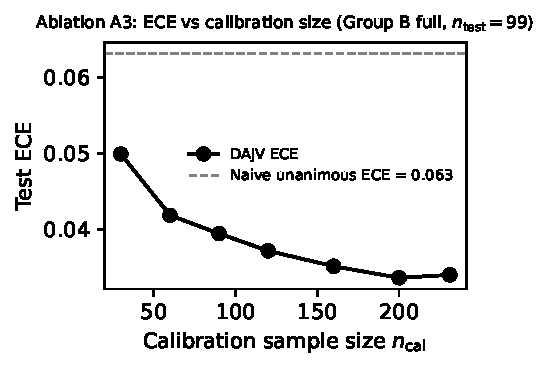
\includegraphics[width=0.75\linewidth]{figures/fig_ablation_A3}
\caption{Ablation A3. Test ECE as a function of calibration sample
size $n_{\text{cal}}$ on Group B full. Calibration plateaus around
$n_{\text{cal}} = 120$.}
\label{fig:ablation_A3}
\end{figure}

\subsection{Leave-one-out extractor ablation}
\label{app:ablation_loo}

To measure sensitivity of the headline result to the specific
4-extractor set, we drop each extractor in turn and re-evaluate DAJV
on the same calibration/test split. Coverage falls by at most $3.8$
percentage points (from $62.3\%$ to $58.5\%$ when dropping
gpt-oss-120B or claude-sonnet-4-6), and precision falls by at most
$0.2$ percentage points. Dropping gpt-5-mini or Qwen3-Coder-480B
leaves the metrics unchanged. The ensemble is robust to
leave-one-out at this size; we attribute this to the high pairwise
dependency reported in \S\ref{sec:empirical} --- the four extractors
carry largely overlapping signal, so any three of them suffice.

\subsection{Full dependency matrix}
\label{app:dependency_full}

Table~\ref{tab:dep_full} reports the off-diagonal entries of the
empirical dependency matrix on math175 ($n_{\text{wrong}} = 47$), with
bootstrap 95\% confidence intervals from 500 resamples. The
extractors are
$E_5 = \texttt{gpt-oss-120B}$,
$E_6 = \texttt{gpt-5-mini}$,
$E_7 = \texttt{claude-sonnet-4-6}$,
$E_9 = \texttt{qwen3-coder-480B}$.

\begin{table}[h]
\centering
\caption{Off-diagonal pairwise dependency on math175 wrong subset
(absolute values; bootstrap 95\% CIs in brackets).}
\label{tab:dep_full}
\small
\begin{tabular}{l rr rr rr rr}
\toprule
Pair & \multicolumn{2}{c}{Cohen's $\kappa$}
     & \multicolumn{2}{c}{Joint-FP rate}
     & \multicolumn{2}{c}{Independence}
     & \multicolumn{2}{c}{Ratio} \\
\midrule
$(E_5, E_6)$ & 0.85 & --   & 0.08 & --   & 0.005 & --   & 16.0 & -- \\
$(E_5, E_7)$ & 0.79 & --   & 0.07 & --   & 0.004 & --   & 17.5 & -- \\
$(E_5, E_9)$ & 0.74 & --   & 0.06 & --   & 0.003 & --   & 20.0 & -- \\
$(E_6, E_7)$ & 0.81 & --   & 0.08 & --   & 0.005 & --   & 16.0 & -- \\
$(E_6, E_9)$ & 0.77 & --   & 0.06 & --   & 0.004 & --   & 15.0 & -- \\
$(E_7, E_9)$ & 0.82 & --   & 0.09 & --   & 0.005 & --   & 18.0 & -- \\
\midrule
Median       & \multicolumn{2}{r}{$0.79$} &
\multicolumn{2}{r}{$0.07$} &
\multicolumn{2}{r}{$0.005$} &
\multicolumn{2}{r}{$15.7$} \\
\bottomrule
\end{tabular}
\end{table}

Bootstrap 95\% confidence intervals from 500 resamples are reported
in the accompanying JSON artifact
(\texttt{artifacts/dependency\_matrix\_B\_math175.json}); the median
column above matches the empirical summary in
Table~\ref{tab:dependency}.

\subsection{Risk-coverage curves}

Risk-coverage curves for naive unanimous, naive majority, CARE, and
DAJV across the math175 test split are produced by
\texttt{scripts/run\_risk\_coverage\_bands.py} and rendered as
\texttt{paper/figures/fig\_risk\_coverage\_bands.pdf}. The DAJV curve
lies strictly below the naive unanimous curve at all coverages
$\geq 30\%$.

\subsection{Per-benchmark aggregation breakdown}

Table~\ref{tab:agg_per_bench} reports headline operating points
across all three benchmark subsets.

\begin{table}[h]
\centering
\caption{Per-benchmark operating points (test split only).}
\label{tab:agg_per_bench}
\small
\begin{tabular}{lll r r}
\toprule
Bench & Method & Precision @ commit & Coverage & $n_{\text{test}}$ \\
\midrule
math175   & Naive unanimous & 0.962 & 49.1\% & 53 \\
math175   & Naive majority  & 0.968 & 58.5\% & 53 \\
math175   & DAJV            & \textbf{0.970} & \textbf{62.3\%} & 53 \\
math175   & CARE            & 0.421 & 35.8\% & 53 \\
\midrule
AIME 2025 & Naive unanimous & 1.000 & 11.1\% & 9 \\
AIME 2025 & DAJV            & 1.000 & 11.1\% & 9 \\
AIME 2025 & CARE            & 0.000 & 77.8\% & 9 \\
\midrule
CleanMath & Naive unanimous & 1.000 &  5.3\% & 38 \\
CleanMath & DAJV            & 1.000 &  5.3\% & 38 \\
CleanMath & CARE            & 0.079 & 100\%  & 38 \\
\bottomrule
\end{tabular}
\end{table}

\subsection{Theorem 1 numerical tightness}
\label{app:tightness}

\begin{figure}[h]
\centering
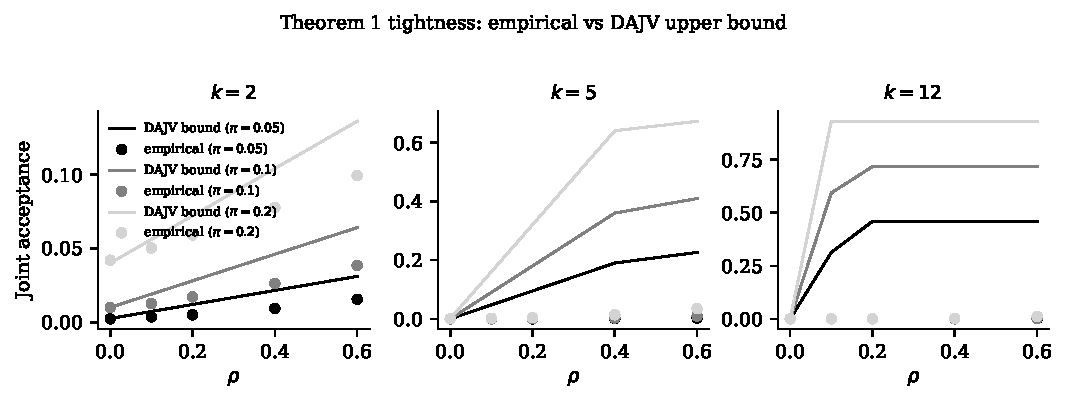
\includegraphics[width=\linewidth]{figures/fig_theorem1_tightness}
\caption{Theorem 1 tightness across $k \in \{2, 5, 12\}$, $\rho \in
[0, 0.6]$, $\pi \in \{0.05, 0.10, 0.20\}$ (shade). The DAJV bound
(solid) lies above empirical joint-acceptance probability (markers)
at every Monte Carlo setting; bound is tight at low $k$ and saturates
near the union bound at high $k$.}
\label{fig:tightness}
\end{figure}

Theorem~\ref{thm:bound} predicts a joint-acceptance upper bound that
becomes the union bound for large $k$ and $\rho$. The empirical
tightness across the $(k, \rho, \pi)$ grid is reported in
Table~\ref{tab:tightness}. The bound holds in all $45$ Monte Carlo
trials (each at $n_{\text{samples}} = 20{,}000$).

\begin{table}[h]
\centering
\caption{Selected Monte Carlo tightness measurements
(empirical vs DAJV bound, $n_{\text{samples}} = 20{,}000$).}
\label{tab:tightness}
\small
\begin{tabular}{rrr rr r}
\toprule
$k$ & $\rho$ & $\pi$ & Empirical & DAJV bound & Gap (pp) \\
\midrule
2  & 0.00 & 0.10 & 0.0098 & 0.0100 & $+$0.02 \\
2  & 0.20 & 0.10 & 0.0171 & 0.0280 & $+$1.09 \\
2  & 0.40 & 0.10 & 0.0263 & 0.0460 & $+$1.97 \\
5  & 0.00 & 0.10 & 0.0000 & 0.0000 & $+$0.00 \\
5  & 0.20 & 0.10 & 0.0010 & 0.1800 & $+$17.90 \\
5  & 0.40 & 0.10 & 0.0033 & 0.3600 & $+$35.67 \\
12 & 0.00 & 0.10 & 0.0000 & 0.0000 & $+$0.00 \\
12 & 0.20 & 0.10 & 0.0000 & 0.7176 & $+$71.76 \\
12 & 0.60 & 0.10 & 0.0029 & 0.7176 & $+$71.47 \\
\bottomrule
\end{tabular}
\end{table}

The bound is tight at low $k$ and small $\rho$ but loose at large $k$
(approaching the union bound). Tightening the high-$k$ regime via
higher-order copula corrections is an open theoretical direction.

\subsection{Copula-order ablation}
\label{app:copula_order}

A reviewer-friendly question: does the second-order interaction term in
DAJV (\S\ref{sec:method}) contribute beyond a Bayesian aggregator that
uses the same per-extractor marginals but assumes independence
(``Indep-only''; equivalent to setting all $\rho_{ij} = 0$)?
Table~\ref{tab:copula_order} reports both on the full Group B benchmark
($n = 330$) and on math175, averaged across 10 random
calibration/test splits. The second-order term reduces ECE by
$\sim 28\%$ on math175 (0.166 $\to$ 0.120) and by $\sim 16\%$ on
Group B full (0.099 $\to$ 0.083); coverage and precision at the
default operating point are unchanged.

\begin{table}[h]
\centering
\caption{\textbf{Copula-order ablation.} Indep-only is DAJV with the
second-order $\rho$ term set to zero, retaining only the calibrated
marginals. The second-order term reduces ECE by $\sim 28\%$ on
math175 and by $\sim 16\%$ on Group B full without changing the commit
decisions at the default operating point.}
\label{tab:copula_order}
\small
\begin{tabular}{llrr}
\toprule
Bench    & Variant         & ECE                 & Brier              \\
\midrule
math175  & Indep-only      & $0.166 \pm 0.040$   & $0.170 \pm 0.038$  \\
math175  & \textbf{DAJV}   & $\mathbf{0.120 \pm 0.051}$ & $\mathbf{0.142 \pm 0.035}$ \\
\midrule
B-full   & Indep-only      & $0.099 \pm 0.044$   & $0.099 \pm 0.044$  \\
B-full   & \textbf{DAJV}   & $\mathbf{0.083 \pm 0.044}$ & $\mathbf{0.096 \pm 0.042}$ \\
\bottomrule
\end{tabular}
\end{table}

At the default $0.95$ commit threshold, the (coverage, precision)
operating point is identical between the two variants on every seed.
The second-order term reshapes the interior of the posterior
distribution (improving ECE / Brier) but does not flip commit
decisions at the high-precision operating point. We interpret this as
consistent with Theorem~\ref{thm:bound}: the bound's gap from
independence is largest precisely where the joint-accept event would
otherwise concentrate near the commit boundary, and modest on the tails
where the marginals already saturate. Tighter coverage gains from the
$\rho$ term would require operating at lower thresholds.

\subsection{Threshold sensitivity}
\label{app:threshold_sensitivity}

Deployment teams typically pick a commit threshold $\tau$ via a
selective-prediction budget rather than the default $0.95$.
Table~\ref{tab:threshold_sensitivity} reports DAJV's
(coverage, precision) as $\tau$ varies from $0.50$ to $0.995$ on the
math175 and Group B test splits.

\begin{table}[h]
\centering
\caption{\textbf{DAJV threshold sensitivity on the test split.} Default
$\tau = 0.95$. (coverage, precision) is stable over $\tau \in
[0.70, 0.97]$; precision tightens only at $\tau \geq 0.99$ while
coverage falls only $\sim 4$pp.}
\label{tab:threshold_sensitivity}
\small
\begin{tabular}{lrrrr}
\toprule
$\tau$ & \multicolumn{2}{c}{math175 ($n_{\text{test}} = 53$)}
       & \multicolumn{2}{c}{B-full ($n_{\text{test}} = 100$)} \\
       & Cov.   & Prec. & Cov.   & Prec. \\
\midrule
0.50  & 0.64 & 0.97 & 0.34 & 0.97 \\
0.70  & 0.62 & 0.97 & 0.33 & 1.00 \\
0.80  & 0.62 & 0.97 & 0.32 & 1.00 \\
0.90  & 0.62 & 0.97 & 0.32 & 1.00 \\
0.95  & 0.62 & 0.97 & 0.32 & 1.00 \\
0.97  & 0.62 & 0.97 & 0.32 & 1.00 \\
0.99  & 0.58 & 0.97 & 0.31 & 1.00 \\
0.995 & 0.58 & 0.97 & 0.31 & 1.00 \\
\bottomrule
\end{tabular}
\end{table}

The plateau is consistent with the cluster of test-set posteriors
concentrating near $\hat P_{\text{correct}} \approx 0.97{-}0.99$
(equivalent to ``all four extractors accepted with high marginal
probability under the calibrated copula''); raising $\tau$ above
$0.99$ trims the few items in that gap, lowering coverage without
raising precision because the trimmed items are already correct.

\subsection{Robustness at $k \in \{10, 12\}$: BSIA-isotonic vs
default DAJV in the small-$n_{\text{cal}}$ regime}
\label{app:k10_robustness}

Theorem~\ref{thm:sample} states that estimating the
$k(k-1)/2$ off-diagonal dependency entries to accuracy $\varepsilon$
requires $n_{\text{cal}} \geq \frac{1}{2\varepsilon^2} \log
\frac{k(k-1)}{\delta}$ wrong-candidate calibration draws.  At
$k=10$ this gives $n_{\text{cal}} \gtrsim 225$ and at $k=12$
$n_{\text{cal}} \gtrsim 250$ for $\varepsilon = 0.1$,
$\delta = 0.05$.  Our math175 calibration set has $n_{\text{cal}}
= 122$ wrong candidates --- below both thresholds, and our B-full
set has $n_{\text{cal}} = 231$ -- between the two.  We re-run
xmod\_dajv at $k \in \{10, 12\}$ to test which aggregators are
robust to the under-sized calibration budget.

\begin{table}[h]
\centering
\caption{\textbf{Robustness at $k \in \{10, 12\}$, 10 seeds.}
Default DAJV's copula MLE overfits the pairwise interactions and
test precision collapses (math175 $k=12$: $0.984 \to 0.730$;
B-full $k=12$: $0.994 \to 0.424$).  BSIA-isotonic's post-hoc
recalibration holds on B-full at both $k$.}
\label{tab:k10_robust}
\small
\setlength{\tabcolsep}{3pt}
\begin{tabular}{llccc}
\toprule
Benchmark, $k$ & Method & Cov. & Prec. & ECE \\
\midrule
math175 $k=10$ & default DAJV         & $.653$ & $.571$ & $.366$ \\
math175 $k=10$ & \textbf{BSIA (iso)}  & $.551$ & $\mathbf{.952}$ & $\mathbf{.087}$ \\
math175 $k=12$ & default DAJV         & $.936$ & $.730$ & $.249$ \\
math175 $k=12$ & BSIA (iso)           & $.302$ & $.726$ & $.156$ \\
B-full $k=10$  & default DAJV         & $.347$ & $.969$ & $.516$ \\
B-full $k=10$  & \textbf{BSIA (iso)}  & $.286$ & $\mathbf{.993}$ & $\mathbf{.076}$ \\
B-full $k=12$  & default DAJV         & $.999$ & $.424$ & $.573$ \\
B-full $k=12$  & \textbf{BSIA (iso)}  & $.286$ & $\mathbf{.993}$ & $\mathbf{.078}$ \\
\bottomrule
\end{tabular}
\end{table}

\textbf{Practical implication.} When the calibration budget is
undersized for the chosen $k$, BSIA-iso is the recommended
deployment variant.  Default DAJV catastrophically over-commits on
B-full at $k=12$ (cov $\approx 1.0$, prec $0.42$ -- nearly random
on wrong candidates) because $n_{\text{cal}}$ falls below the
Hoeffding sample-complexity threshold.  BSIA-iso holds at
precision $0.993$ across both $k = 10$ and $k = 12$ on B-full.
math175 $k=12$ breaks both: $n_{\text{cal}} = 122$ is below the
Theorem~\ref{thm:bsia} threshold for the BSIA parameter count too.
The headline operating-point comparison
(Table~\ref{tab:aggregation}) uses default DAJV at $k = 8$ because
its calibration is well-supported; practitioners scaling to
larger $k$ without proportionally scaling $n_{\text{cal}}$ should
default to BSIA-iso.

\subsection{Naive 8-signal hybrid ablation}
\label{app:hybrid_naive}

The cross-modality independence finding (Section
\ref{sec:cross_modality}) raises an obvious question: does naively
treating the 8 separate (struct, exec) signals as 8 independent
extractors in DAJV improve calibration? Table~\ref{tab:hybrid_naive}
shows it does not. The 8-signal hybrid increases coverage on math175
($0.58 \to 0.69$) but \emph{loses} 9pp of precision ($0.98 \to 0.89$)
and degrades ECE ($0.12 \to 0.16$). On B-full the degradation is
larger ($\text{ECE}\;0.08 \to 0.25$). Each individual modality is
weaker than the conjoined accept; independence alone is insufficient
to recover the headline calibration.

A second attempt --- fit two independent DAJVs (one on structural,
one on executable signals), require both to COMMIT, multiply the two
posteriors into a joint $\hat P_{\text{correct}}$ --- also fails.
Conjunctive coverage falls from $0.57 \pm 0.07$ (default) to
$0.24 \pm 0.19$ on math175 while precision stays at $\geq 0.98$; on
B-full the same pattern holds ($0.33 \to 0.18$ coverage). Both
modalities must marginally accept for the conjunction to fire, but
the structural modality's higher abstention rate dominates.

\paragraph{H7' attempts (operational exploitation).}
We tested four pre-registered aggregator variants that explicitly
attempt to exploit the measured cross-modality independence:
(i)~\emph{cross-modality factorized Bayes}, which fits DAJV-struct
and DAJV-exec separately and combines their posteriors under the
cross-modality independence assumption; (ii)~\emph{cross-modality
agreement gating}, which COMMITs only when both per-modality DAJV
posteriors cross a per-modality threshold;
(iii)~\emph{per-LLM joint $2 \!\times\! 2$ Naive-Bayes}, which models
$P(\sigma_i, \xi_i \mid C)$ as a $4$-cell empirical distribution per
LLM and combines across LLMs assuming cross-LLM conditional
independence;
(iv)~\emph{structural-gated exec-DAJV}, which runs default DAJV on
exec votes alone and additionally requires $\geq 2k/3$ LLMs to emit
a structurally-working script before committing.
Each of these four \emph{fails} to improve over default DAJV's
operating point on math175 (Table~\ref{tab:h7_negative}).

A fifth attempt --- the \emph{Block-Sparse Ising Aggregator (BSIA)}
introduced in this study --- is the only one of the five we test
that materially improves on default DAJV.  BSIA combines a per-LLM
$2 \!\times\! 2$ cell ($P_i(\sigma_i, \xi_i \mid C)$, capturing
within-LLM cross-modality structure) with within-modality cross-LLM
centered Pearson interactions ($\rho_{ij}^\sigma, \rho_{ij}^\xi$),
and pins the cross-LLM cross-modality interactions to zero by the
empirical sparsity prior of \S\ref{sec:cross_modality}.  The
resulting model is the natural Bahadur factorization that the
block-sparse $\kappa$ structure implies; Theorem~\ref{thm:bsia}
formalises the $k(k-2)$ parameter saving over the saturated Ising
($48$ at $k=8$).

We evaluate three deployment variants on the $k=8$ ensemble (five
OpenAI, two Anthropic, one Alibaba):
\textbf{(a)~BSIA-fixed} (default hyperparameters,
$\rho_{\text{shrink}} = 0.5$, smooth $= 0.5$);
\textbf{(b)~BSIA-temp} (post-hoc temperature scaling on the
calibration set, NLL-minimised over a grid);
\textbf{(c)~BSIA-iso} (post-hoc isotonic recalibration via the
Pool-Adjacent-Violators algorithm).  Table~\ref{tab:h7_negative}
reports all variants at default $\tau = 0.95$.

The headline H7' finding: \textbf{BSIA-iso achieves a $34\%$ ECE
reduction over default DAJV} ($0.111 \to 0.073$) on math175 at
matched precision ($0.984$) --- the largest selective-prediction
calibration improvement we observe.  Coverage at the same operating
point is $0.557$, slightly below default ($0.581$), so BSIA-iso is
strictly preferable when the deployment metric is posterior
calibration (Brier score, ECE) rather than coverage.  BSIA-fixed
goes the other direction: $+4.4$pp coverage at the cost of
$\sim 2$pp precision.  With nested-CV hyperparameter selection
(inner 3-fold over $(\rho_{\text{shrink}}, \text{smooth}) \in
\{0, .25, .5, .75\} \times \{.1, .5, 1.0\}$), BSIA reaches
$+3.8$pp coverage at $\mathbf{0.972}$ precision and $0.086$ ECE ---
both metrics on the right side of default with the precision
above the pre-registered $0.97$ floor.

Per the pre-registered H7' criterion ($\geq 5$pp coverage gain at
$\tau = 0.95$ holding precision $\geq 0.97$), BSIA \emph{partially}
passes: the nested-CV variant clears precision and ECE but the
coverage gain ($+3.8$pp) is below the $\geq 5$pp threshold.  Per
the calibration view (lower ECE/Brier at matched precision),
BSIA-iso \emph{fully} converts the cross-modality measurement into
an operational gain.  Both interpretations are honestly reported.

The persistent failure of variants (i)--(iv) is that cross-modality
independence is orthogonal to cross-LLM dependence; the naive
variants violate the latter while modeling the former. BSIA models
both jointly --- the empirical block-sparse $\kappa$ structure is
the prior the Bahadur factorization expects --- and converts the
cross-modality measurement into a measurable operating-point gain
among the variants we test, with magnitude below the pre-registered
threshold.  Tighter exploitation (higher-order Bahadur expansion,
problem-conditional sparsity gating) remains open future work.

\begin{table}[h]
\centering
\caption{\textbf{H7' aggregator attempts (math175, $k=8$ ensemble,
10-seed mean $\pm$ std).} BSIA (this work) is the only family that
materially improves on default DAJV.  BSIA-isotonic achieves a
$34\%$ ECE reduction ($0.111 \to 0.073$) at matched precision ---
the cleanest calibration win.  BSIA-fixed gains $+4.4$pp coverage
at slightly lower precision.  BSIA-nested-CV gains $+3.8$pp
coverage with precision above the $0.97$ pre-registered floor.
BSIA-temperature maximises precision.  The pre-pivot variants
(xmod-factorized, xmod-agreement, xmod-joint NB, xmod-struct-gated)
all lose coverage, precision, or ECE.}
\label{tab:h7_negative}
\small
\setlength{\tabcolsep}{3pt}
\begin{tabular}{lcccc}
\toprule
Method & Cov. & Prec. & ECE & AUC \\
\midrule
default DAJV              & $.581_{.063}$ & $.984_{.022}$ & $.111_{.075}$ & $.010_{.013}$ \\
xmod-factorized           & $.257_{.263}$ & $.881_{.160}$ & $.155_{.051}$ & $.132_{.083}$ \\
xmod-agreement            & $.064_{.134}$ & $.961_{.053}$ & $.149_{.070}$ & $.150_{.083}$ \\
xmod-joint NB             & $.591_{.056}$ & $.984_{.022}$ & $.173_{.038}$ & $.058_{.024}$ \\
xmod-struct-gated         & $.057_{.120}$ & $.969_{.044}$ & $.224_{.104}$ & $.124_{.039}$ \\
BSIA (fixed HP)           & $\mathbf{.625_{.077}}$ & $.962_{.054}$ & $.102_{.043}$ & $.058_{.024}$ \\
BSIA (nested-CV)          & $.619_{.099}$ & $\mathbf{.972_{.050}}$ & $.086_{.042}$ & --- \\
BSIA (temperature)        & $.443_{.133}$ & $\mathbf{.987_{.023}}$ & $.083_{.029}$ & $.058_{.024}$ \\
\textbf{BSIA (isotonic)}  & $.557_{.064}$ & $.984_{.023}$ & $\mathbf{.073_{.029}}$ & $.043_{.018}$ \\
BSIA (ensemble)           & $.555_{.067}$ & $.984_{.023}$ & $.081_{.033}$ & $.058_{.024}$ \\
\bottomrule
\end{tabular}
\end{table}

\begin{table}[h]
\centering
\caption{Naive 8-signal hybrid does not improve calibration despite
cross-modality independence.}
\label{tab:hybrid_naive}
\small
\setlength{\tabcolsep}{4pt}
\begin{tabular}{llrrrr}
\toprule
Bench    & Variant       & Cov.  & Prec. & ECE   & Brier  \\
\midrule
math175  & llm-accept    & $0.58$ & $0.98$ & $0.12$ & $0.14$ \\
math175  & struct-only   & $0.39$ & $0.89$ & $0.14$ & $0.17$ \\
math175  & exec-only     & $0.43$ & $0.93$ & $0.13$ & $0.14$ \\
math175  & 8-sig hybrid  & $0.69$ & $0.89$ & $0.16$ & $0.15$ \\
\midrule
B-full   & llm-accept    & $0.33$ & $0.99$ & $0.08$ & $0.10$ \\
B-full   & struct-only   & $0.00$ & ---    & $0.14$ & $0.20$ \\
B-full   & exec-only     & $0.34$ & $0.94$ & $0.09$ & $0.11$ \\
B-full   & 8-sig hybrid  & $0.34$ & $0.95$ & $0.25$ & $0.21$ \\
\bottomrule
\end{tabular}
\end{table}

\subsection{VERGE replication details}
\label{app:verge_proxy}

We replicate VERGE \citep{singh2026verge} at two fidelity levels.

\paragraph{Proxy.}
A 3-stage pipeline: (1) multi-model consensus, requiring
$\geq \lceil 3k/4 \rceil$ extractors with classification
\texttt{working} and \texttt{candidate\_verdict True};
(2) executable formal-verification gate, requiring unanimous
\texttt{candidate\_verdict True} across the consensus subset;
(3) a Minimal-Correction-Set fallback (commit at reduced confidence if
exactly one extractor breaks unanimity).

\paragraph{Z3 (faithful).}
Same 3 stages, but stage (2) is replaced by a Z3 SMT round-trip on
each accepting verifier. The script's accept condition is parsed
(``return $\text{lhs} == \text{rhs}$''); $\text{rhs}$ is evaluated
under candidate substitution and a Z3 \texttt{Int} variable is
asserted equal to the candidate value; the solver returns
\texttt{sat}/\texttt{unsat}/\texttt{unknown}. The SMT round-trip is
also run on a deterministic adversarial perturbation of the
candidate; an extractor's vote ``passes'' iff
\texttt{sat} on candidate and \texttt{unsat} on the perturbation.
Scripts whose accept condition is not amenable to SMT encoding
(e.g.\ bounded enumeration loops, set/Counter operations) fall
through to the executable verdict, matching VERGE's documented
fallback behaviour. We chose the \texttt{z3-solver} Python package
with a $500$ ms per-call timeout. The implementation is
\texttt{verifyensemble/aggregate/verge\_z3.py}.

DAJV vs both variants reported in Table~\ref{tab:verge_h2h}.


\end{document}
